

\documentclass[a4paper,twoside]{article}

\usepackage{epsfig}
\usepackage{subfigure}
\usepackage{calc}
\usepackage{amssymb}
\usepackage{amstext}
\usepackage{amsmath}
\usepackage{amsthm}
\usepackage{graphicx}
\usepackage{multicol}
\usepackage{pslatex}
\usepackage{apalike}
\usepackage{SciTePress}
\usepackage[small]{caption}

\subfigtopskip=0pt
\subfigcapskip=0pt
\subfigbottomskip=0pt


\newcommand{\fnceval}{function evaluation}
\newcommand{\fncevals}{function evaluations}

\newcommand{\fe}{function evaluation}
\newcommand{\fes}{function evaluations}

\newcommand{\fnces}{function evaluations}





\newcommand{\pfe}{{probFE}}


\newcommand{\vi}{VI}

\newcommand{\dyp}{DP}

\newcommand{\mdp}{MDP}
\newcommand{\mdps}{MDPs}

\newcommand{\pso}{{\sc pso}}
\newcommand{\spso}{{\sc s-pso}}
\newcommand{\cfe}{{\sc gr-pso}}

\newcommand{\fips}{{\sc fips}}


\newcommand{\alg}{algorithm}
\newcommand{\algs}{algorithms}
\newcommand{\Algs}{Algorithms}

\newcommand{\psoalg}{{\sc pso} algorithm}



\newcommand{\prt}{particle}
\newcommand{\prts}{particles}
\newcommand{\Prts}{Particles}


\newcommand{\gb}{global best}
\newcommand{\gbs}{global bests}
\newcommand{\pb}{personal best}
\newcommand{\pbs}{personal bests}

\newcommand{\gbn}{\emph{gbest}}
\newcommand{\ring}{\emph{ring}}

\newcommand{\topo}{topology}


\newcommand{\iter}{iteration}
\newcommand{\iters}{iterations}




\begin{document}

\title{GREEN-PSO: Conserving Function Evaluations \\ in Particle Swarm Optimization}

\author{\authorname{Stephen M. Majercik\sup{1}}
\affiliation{\sup{1}Department of Computer Science, Bowdoin College, Brunswick, Maine, USA}
\email{smajerci@bowdoin.edu}
}


\keywords{particle swarm optimization; swarm intelligence.}

\abstract{In the Particle Swarm Optimization (\pso) algorithm, the expense of evaluating the objective function can make it difficult, or impossible, to use this approach effectively; reducing the number of necessary \fncevals\ would make it possible to apply the \pso\ algorithm more widely. Many function approximation techniques have been developed that address this issue, but an alternative to function \emph{approximation} is function \emph{conservation}. We describe {\sc green-pso} (\cfe), an algorithm that, given a fixed number of \fncevals, conserves those \fncevals\ by probabilistically choosing a subset of particles smaller than the entire swarm on each iteration and allowing only those particles to perform \fncevals. The ``surplus'' of \fncevals\ thus created allows a greater number of particles and/or iterations. In spite of the loss of information resulting from this more parsimonious use of \fncevals, \cfe\ performs as well as, or better than, the standard \psoalg\ on a set of six benchmark functions, both in terms of the rate of error reduction and the quality of the final solution.}

\onecolumn \maketitle \normalsize \vfill




\section{\uppercase{Introduction}}
\label{s:intro}


Swarm intelligence is a natural phenomenon in which complex behavior emerges from the collective activities of a large number of simple individuals who interact with each other and their environment in very limited ways. A number of swarm  based optimization techniques have been developed, among them Particle Swarm Optimization (\pso).  \pso, introduced by Kennedy and Eberhart, is loosely based on the phenomenon of birds flocking~\cite{kennedy95}. Virtual particles ``fly'' through the solution space in search of high quality solutions. The search trajectory of a particle is influenced by both the best solution it has found so far (personal best) and the best solution that has been found so far in its neighborhood; that solution will be a \emph{global best} if the neighborhood is the entire swarm (as in the original \pso\ \alg), or a \emph{local best} if the neighborhood is a strict subset of the swarm. The algorithm iteratively updates the velocities and positions of the particles guided by the personal bests and the neighborhood bests, converging on a (hopefully) global optimum. \pso\ is one of the most widely used swarm-based algorithms and has been applied successful to many real world problems~\cite{poli07}. 
Many variants of the \pso\ \alg\ have been proposed~\cite{sedighizadeh09}.

The trajectories of the particles in \pso\ depend critically on calculating the value of the objective function at every position each particle visits.  In the standard \pso\ \alg, every particle does a function evaluation on every iteration in order to determine the fitness of the candidate solution at the particle's new position. A typical \pso\ \alg\ uses at least 20-40 particles and thousands of iterations to find even a suboptimal (but acceptable) solution, and this high number of \fes\ can be difficult to achieve in real world applications if the objective function is expensive to compute, in terms of time and/or money.  For example, evaluating the effectiveness of a complex control mechanism that a \pso\ \alg\ is trying to optimize might involve running a simulation that takes several hours.  

A common way of addressing this problem is to use \emph{function approximation}, which can take many forms: response surface methods, radial basis functions, Kriging (DACE models), Gaussian process regression, support vector machines, and neural networks~\cite{santana-quintero08}.  Another approximation technique is \emph{fitness inheritance}, in which the objective function value, or fitness, of an individual is approximated based on the fitnesses of one or more other individuals designated as ``parents''\cite{reyes-sierra07}.

Instead of using less expensive---but possibly less effective---approximations of the function, an \alg\  could perform fewer exact evaluations of the function, thereby conserving this resource.  This is the approach adopted by {\sc green-pso} (\cfe), the algorithm we present here.  \cfe\ demonstrates that performance comparable to or, in some cases, better than that of the standard \pso\ \alg\ can be achieved by permitting only a subset of the particles in the swarm to do \fncevals\ during each iteration, and using the conserved \fncevals\ to increase the number of particles in the swarm and/or the number of iterations that are possible, given a fixed number of \fncevals.  

In Section~\ref{s:pso}, we describe the basic \pso\ \alg\ and present the \cfe\ \alg.  We describe and discuss the results of our experiments in Section~\ref{s:experiments}.  We discuss related work in Section~\ref{s:related-work}, and conclude with some ideas for future work in Section~\ref{s:future-work}.



\section{\uppercase{PSO and GR-PSO}}
\label{s:pso}


\subsection{Standard PSO}

The standard \pso\ \alg\ uses a swarm of particles to iteratively search a $d$-dimensional solution space for good solutions, guided by their own experience and that of the swarm. The number of particles in the swarm is fixed and the position and velocity of each particle $i$, $\vec{x}_{i}$ and $\vec{v}_{i}$, respectively, are initialized randomly.  Particle $i$ remembers the best solution it has found so far, $\vec{p}_{i}$, and the best solution found so far by the particles in particle $i$'s neighborhood, $\vec{g}_{i}$. (In the original \pso\ \alg, the neighborhood of every particle is the entire swarm.) The velocity $\vec{v}_{i}$ of particle $i$ is updated during each iteration such that its motion is biased toward both $\vec{p}_{i}$ and $\vec{g}_{i}$, and the new velocity is used to update its position $\vec{x}_{i}$.  There are a number of basic \pso\ \algs.  For purposes of comparison, we adopt the \pso\ \alg\ with a \emph{constriction coefficient} $\chi$ and \emph{velocity limits} as described in~\cite{poli07}, which we reproduce here with minor changes.  The velocity and position update equations are:
\begin{align} 
\label{pso-update-eqs}
    \vec{v}_{i} & \leftarrow \chi ( \vec{v}_{i} + \vec{U}(0,\phi_{1}) \otimes (\vec{p}_{i} - \vec{x}_{i}) + \vec{U}(0,\phi_{2}) \otimes (\vec{g}_{i} - \vec{x}_{i}))  \\ 
\vec{x}_{i}    & \leftarrow \vec{x}_{i} + \vec{v}_{i} 
\end{align} 
where:
\begin{itemize}
\item
$\phi_1$ and $\phi_2$, the \emph{acceleration coefficients} that scale the attraction of particle $i$ to $\vec{p}_{i}$ and $\vec{g}_{i}$, respectively, are equal,
\item
$\vec{U}(0,\phi_{i})$ is a vector of real random numbers uniformly distributed in $[0,\phi_{i}]$, which is randomly generated at each iteration for each particle, and
\item
$\otimes$ is component-wise multiplication.
\end{itemize}
The value of the constriction coefficient $\chi$ is:
$\frac{2}{\phi - 2 + \sqrt{\phi^{2} - 4 \phi}}$
where $\phi = \phi_1 + \phi_2 = 4.1$, giving $\chi$ a value of approximately 0.7298.
Finally, each component $\vec{v}_{i}$ is restricted to a range $[V_{\mbox{\scriptsize min}}, V_{\mbox{\scriptsize max}}]$, where $V_{\mbox{\scriptsize min}}$ and $V_{\mbox{\scriptsize max}}$ are the minimum and maximum values of the search space and are identical for each dimension. 



\subsection{GR-PSO}

The \pso\ \alg\ is often motivated by referencing the human decision-making process, in which an individual, confronted with a problem, makes a decision based partially on her own experience solving that problem in the past 
and partially on the experience of others who have solved that problem before.
Extending that analogy, we suggest that, while trying to improve the best solution she has found in the past, she may suspend evaluation of her efforts for a period of time, in order to conserve the resources that would be required to evaluate the solution.  A second goal might be to prevent evaluating a new solution prematurely and possibly rejecting it before its value can be accurately assessed.

\cfe\ models these goals in the following way.  \cfe\ operates like \spso, except that each particle, after calculating a new velocity and changing its position according to that velocity, performs a function evaluation on its new position with some probability \emph{\pfe}, where $0.0 <$ \pfe\ $< 1.0$. This means that on every iteration, the expected number of particles doing a \fe\ is ($n \ \times$ \pfe), where $n$ is the number of particles in the swarm, so the expected number of iterations is (numFEs/($n \ \times$ \pfe)), where numFEs is the total number of \fncevals\ available. 
This allows the swarm to use more particles for the same number of iterations, or more iterations for the same number of particles. 
See Figure~\ref{f:pseudocode} for pseudocode for \cfe.


\begin{figure}[h]
\begin{tabbing}
xx\=xx\=xx\=xx\=xx\=xx\=xx\=xx\=xx\=xx\=xx\=xx\=\kill
$\mbox{{\sc {\bf BEGIN}}} $ \\
\> Initialize swarm \\
\> {\bf while} (numFunctionEvaluations $\leq$ 10,000) \\
\> \> {\bf for} each particle: \\
\> \> \> Calculate velocity and move\\
\> \> \> {\bf if} (randomDouble $<$ probFE) \\
\> \> \> \> Evaluate new position and update bests \\
\> \> \> {\bf end-if} \\
\> \> {\bf end-for} \\
\> {\bf end-while}  \\
$\mbox{{\sc {\bf END}}} $ \\
\end{tabbing}
\vspace{-0.25in}
\caption{Pseudocode for \cfe.}
\label{f:pseudocode}
\end{figure}





\section{\uppercase{Experimental Results}}
\label{s:experiments}

We tested \cfe\ on six standard benchmark functions: Sphere ($f_1$), Rosenbrock ($f_2$), Ackley ($f_3$), Griewank ($f_4$), Rastrigin ($f_5$), and Penalized Function P16 ($f_6$) ($f_i$ identifiers used in Tables~\ref{t:gbest-data} and \ref{t:mann-whitney-data}).  See \cite{bratton07} for the function definitions.
 Sphere and Rosenbrock are uni-modal functions, while Ackley, Griewank, Rastrigin, and Penalized Function P8 are multi-modal functions with many local optima. The optimum (minimum) value for all of these functions is 0.0.
 We randomly shifted the location of the optima away from the center of the search space in order 
to avoid the tendency of \pso\ \algs\ to converge to the center~\cite{monson05}.


We tested each of these functions in 30 dimensions.  We used the \gbn\ \topo, in which the neighborhood for each particle is the entire swarm, for both \cfe\ and \spso. We fixed the number of \fncevals\ at 10,000 and tested over a range of number of particles (10, 20, 50, 100, 200) and a range of values for \pfe\ (0.9, 0.8, \ldots, 0.1).  We measured the mean and standard deviation of the best (lowest) function value found and the median error every 2,000 \fes\ (to avoid the effect of outliers). 

A note on our choice of topologies:  It seems likely that \cfe\ works, at least in part, because, by delaying the discovery of new global bests, it weakens the tendency of the \gbn\ \topo\ to produce early convergence on a local minimum. Topologies with smaller neighborhoods, such as the \ring\ \topo\ (in which the particles can be viewed as being arranged in a ring, and the neighbors of each particle are just the two particles on either side of it) also improve performance by slowing the propagation of the global best. 
And, in fact, it was the case that, using the \ring\ \topo, \cfe\ did not provide the same performance gains over \spso\ as it did with the \gbn\ \topo.  Thus, it would seem that a more appropriate comparison would be between \cfe\ using the \gbn\ \topo\ and \spso\ using the \ring\ \topo. The improved performance of the \ring\ \topo\ over the \gbn\ \topo, however, is obtained only with a sufficient number of iterations and our limit of 10,000 \fncevals\ did not allow sufficient iterations for the \ring\ \topo's benefits to materialize.  In fact, while \spso\ with the \ring\ \topo\ outperformed \spso\ with the \gbn\ \topo\ when 200,000 \fncevals\ were allowed, \spso\ with the \gbn\ \topo\ outperformed \spso\ with the \ring\ \topo\ when only 10,000 \fncevals\ were allowed.  For this reason, we feel that the appropriate comparison for \cfe\ with the \gbn\ \topo\ is still \spso\ with the \gbn\ \topo, and we report those results.

Initial tests suggested that 10 particles are unable to explore the space sufficiently, even given the additional iterations provided by a \pfe\ of less than 1.0, and that swarms of 100 or 200 particles reduce the number of iterations (given the fixed number of \fncevals) to unacceptable levels, in spite of the additional iterations provided by a \pfe\ of less than 1.0. Thus, we confined further tests to 20-particle and 50-particle swarms.  Initial tests of the \spso\ \alg\ over the same range of number of particles indicated that 20-particle and 50-particle swarms were best for that \alg\ as well, for similar reasons.



\begin{table*}
\begin{tabular}{|| l | l | r | r | r | r | r | r ||}

\hline \hline \hline

  Func-  &              & \multicolumn{1}{c|}{Mean Function Value}  & \multicolumn{5}{c||}{Median Error (121 runs) for Num of Function Evaluations}\\ 
                                                                      \cline{4-8}
  tion   &  Algorithm   & \multicolumn{1}{c|}{(Standard Deviation)} & 2,000 & 4,000 & 6,000 & 8,000 & 10,000 \\

\hline \hline 

%SPHERE
$f_1$   &  CPSO-20-0.2    &  {\bf 5.44e-07} (2.36e-06)         &  {\bf 1.47e+02}         &  {\bf 5.43e-01}         &  {\bf 1.88e-03}         &  {\bf 9.45e-06}         &  {\bf 3.09e-08}  \\
    \cline{2-8}
        &  CPSO-20-0.1    &  {\bf \emph{4.91e-08}} (2.11e-07)  &  {\bf 8.61e+01}         &  {\bf 1.92e-01}         &  {\bf 4.66e-04}         &  {\bf 1.01e-06}         &  {\bf 2.83e-09}  \\
    \cline{2-8}    
        &  CPSO-20-0.05   &  {\bf 1.31e-07} (1.22e-06)         &  {\bf \emph{5.66e+01}}  &  {\bf \emph{1.10e-01}}  &  {\bf \emph{2.48e-04}}  &  {\bf \emph{5.81e-07}}  &  {\bf \emph{1.24e-09}}  \\
    \cline{2-8}
        &  CPSO-50-0.2    &  1.77e-03 (2.40e-03)               &  8.61e+02               &  2.86e+01               &  8.01e-01               &  2.36e-02               &  8.25e-04  \\
    \cline{2-8}
        &  CPSO-50-0.1    &  1.65e-04 (2.04e-04)               &  5.76e+02               &  1.25e+01               &  2.49e-01               &  5.05e-03               &  8.85e-05  \\
    \cline{2-8}
        &  CPSO-50-0.05   &  3.70e-05 (4.74e-05)               &  4.41e+02               &  7.08e+00               &  8.35e-02               &  1.54e-03               &  1.95e-05  \\
\hline \hline
        &  SPSO-20        &  5.42e-03 (1.28e-02)               &  6.70e+02               &  2.15e+01               &  9.19e-01               &  3.08e-02               &  9.94e-04  \\
    \cline{2-8}
        &  SPSO-50        &  1.14e+00 (1.47e+00)               &  2.93e+03               &  3.67e+02               &  4.73e+01               &  5.66e+00               &  6.93e-01  \\

\hline \hline \hline

% ROSENBROCK
$f_2$   &  CPSO-20-0.2    &  3.77e+01 (2.42e+01)               &  {\bf 8.88e+01}         &  {\bf 3.08e+01}         &  {\bf 2.75e+01}         &  {\bf 2.67e+01}         &  2.62e+01  \\
    \cline{2-8} 
        &  CPSO-20-0.1    &  3.45e+01 (2.47e+01)               &  {\bf \emph{7.15e+01}}  &  {\bf 2.89e+01}         &  {\bf 2.72e+01}         &  {\bf 2.66e+01}         &  {\bf 2.61e+01}  \\
    \cline{2-8}
        &  CPSO-20-0.05   &  3.57e+01 (2.56e+01)               &  {\bf 7.66e+01}         &  {\bf \emph{2.82e+01}}  &  {\bf \emph{2.70e+01}}  &  {\bf \emph{2.65e+01}}  &  {\bf 2.61e+01} \\
    \cline{2-8}
        &  CPSO-50-0.2    &  {\bf 3.11e+01} (1.57e+01)         &  1.35e+02               &  3.98e+01               &  2.84e+01               &  2.72e+01               &  2.67e+01 \\
    \cline{2-8}
        &  CPSO-50-0.1    &  3.52e+01 (2.10e+01)               &  1.29e+02               &  5.30e+01               &  2.85e+01               &  2.74e+01               &  2.68e+01 \\
    \cline{2-8}
        &  CPSO-50-0.05   &  {\bf \emph{3.06e+01}} (1.67e+01)  &  1.12e+02               &  3.28e+01               &  2.79e+01               &  2.71e+01               &  2.65e+01 \\
\hline \hline
        &  SPSO-20        &  {\bf 3.24e+01} (1.80e+01)         &  1.28e+02               &  4.82e+01               &  2.89e+01               &  2.70e+01               &  {\bf \emph{2.60e+01}} \\
    \cline{2-8} 
        &  SPSO-50        &  4.04e+01 (2.44e+01)               &  2.86e+02               &  9.94e+01               &  4.36e+01               &  3.00e+01               &  2.80e+01 \\

\hline \hline \hline

% ACKLEY
$f_3$   &   CPSO-20-0.2   &  9.93e+00 (8.00e+00)               &  {\bf 7.85e+00}         &  5.57e+00               &  5.53e+00               &  5.53e+00               &  5.53e+00  \\
    \cline{2-8}
        &   CPSO-20-0.1   &  9.92e+00 (7.50e+00)               &  {\bf \emph{7.78e+00}}  &  6.16e+00               &  6.13e+00               &  6.13e+00               &  6.13e+00  \\
    \cline{2-8}
        &   CPSO-20-0.05  &  1.17e+01 (7.36e+00)               &  1.21e+01               &  1.04e+01               &  1.02e+01               &  1.02e+01               &  1.02e+01  \\
    \cline{2-8} 
        &   CPSO-50-0.2   &  {\bf \emph{6.04e+00}} (8.72e+00)  &  8.60e+00               &  {\bf 3.56e+00}         &  {\bf \emph{1.76e+00}}  &  {\bf \emph{1.35e+00}}  &  {\bf \emph{1.34e+00}}  \\
    \cline{2-8}
        &   CPSO-50-0.1   &  {\bf 7.48e+00} (9.23e+00)         &  8.91e+00               &  {\bf \emph{3.33e+00}}  &  {\bf 1.94e+00}         &  {\bf 1.65e+00}         &  {\bf 1.65e+00}  \\
    \cline{2-8}
        &   CPSO-50-0.05  &  8.54e+00 (9.18e+00)               &  {\bf 8.41e+00}         &  {\bf 3.40e+00}         &  {\bf 2.25e+00}         &  {\bf 2.02e+00}         &  {\bf 2.01e+00}  \\
\hline \hline
        &   SPSO-20       &  9.39e+00 (8.15e+00)               &  9.36e+00               &  5.07e+00               &  4.59e+00               &  4.38e+00               &  4.38e+00  \\
    \cline{2-8}
        &   SPSO-50       &  {\bf 8.35e+00} (9.08e+00)         &  1.30e+01               &  6.78e+00               &  4.08e+00               &  2.85e+00               &  2.35e+00  \\

\hline \hline \hline

% GRIEWANK             
$f_4$   &  CPSO-20-0.2    &  3.78e-02 (6.66e-02)               &  {\bf 2.01e+00}         &  {\bf 4.60e-01}         &  {\bf 2.65e-02}         &  {\bf 1.72e-02}         &  1.72e-02 \\
    \cline{2-8} 
        &  CPSO-20-0.1    &  8.09e-02 (2.95e-01)               &  {\bf \emph{1.59e+00}}  &  {\bf 2.54e-01}         &  {\bf 3.55e-02}         &  2.70e-02               &  2.70e-02 \\
    \cline{2-8}
        &  CPSO-20-0.05   &  6.67e-02 (1.63e-01)               &  {\bf 1.69e+00}         &  {\bf \emph{1.94e-01}}  &  {\bf \emph{2.56e-02}}  &  {\bf 2.21e-02}         &  2.21e-02 \\
    \cline{2-8}
        &  CPSO-50-0.2    &  {\bf \emph{1.72e-02}} (1.97e-02)  &  9.26e+00               &  1.28e+00               &  8.24e-01               &  7.14e-02               &  {\bf 1.23e-02} \\
    \cline{2-8}
        &  CPSO-50-0.1    &  {\bf 1.74e-02} (2.54e-02)         &  7.39e+00               &  1.11e+00               &  4.50e-01               &  2.60e-02               &  {\bf 1.08e-02} \\
    \cline{2-8}
        &  CPSO-50-0.05   &  {\bf 1.85e-02} (2.17e-02)         &  4.81e+00               &  1.06e+00               &  1.92e-01               &  {\bf \emph{1.53e-02}}  &  {\bf \emph{9.93e-03}} \\
\hline \hline
        &  SPSO-20        &  9.02e-02 (1.67e-01)               &  6.65e+00               &  1.18e+00               &  5.17e-01               &  7.28e-02               &  3.99e-02 \\
    \cline{2-8}
        &  SPSO-50        &  6.93e-01 (2.32e-01)               &  3.16e+01               &  4.11e+00               &  1.38e+00               &  1.06e+00               &  7.09e-01 \\

\hline \hline \hline


% RASTRIGIN       
$f_5$   &  CPSO-20-0.2    &  1.02e+02 (4.88e+01)               &  {\bf \emph{1.07e+02}}  &  {\bf 9.08e+01}         &  9.05e+01               &  9.05e+01               &  9.05e+01 \\
    \cline{2-8} 
        &  CPSO-20-0.1    &  1.18e+02 (7.05e+01)               &  {\bf 1.17e+02}         &  9.66e+01               &  9.65e+01               &  9.65e+01               &  9.65e+01 \\
    \cline{2-8}
        &  CPSO-20-0.05   &  1.25e+02 (8.01e+01)               &  {\bf \emph{1.07e+02}}  &  9.46e+01               &  9.45e+01               &  9.45e+01               &  9.45e+01 \\
    \cline{2-8}
        &  CPSO-50-0.2    &  {\bf \emph{7.53e+01}} (3.35e+01)  &  1.83e+02               &  9.58e+01               &  {\bf 7.42e+01}         &  {\bf \emph{6.71e+01}}  &  {\bf \emph{6.57e+01}} \\
    \cline{2-8}
        &  CPSO-50-0.1    &  {\bf 8.16e+01} (3.44e+01)         &  1.65e+02               &  {\bf 9.30e+01}         &  {\bf 7.82e+01}         &  {\bf 7.37e+01}         &  7.36e+01 \\
    \cline{2-8}
        &  CPSO-50-0.05   &  8.49e+01 (4.69e+01)               &  1.40e+02               &  {\bf \emph{8.42e+01}}  &  {\bf \emph{7.33e+01}}  &  {\bf 7.17e+01}         &  {\bf 7.16e+01} \\
\hline \hline
        &  SPSO-20        &  8.80e+01 (3.17e+01)               &  1.70e+02               &  9.87e+01               &  8.59e+01               &  8.36e+01               &  8.36e+01 \\
    \cline{2-8}
        &  SPSO-50        &  {\bf 7.65e+01} (2.57e+01)         &  2.61e+02               &  1.71e+02               &  1.16e+02               &  8.73e+01               &  {\bf 7.35e+01} \\

\hline \hline \hline






% PENAL 2  (P16)    
$f_6$   &  CPSO-20-0.2    & 4.71e-01 (1.01e+00)                &  {\bf 5.70e+03}         &  {\bf 1.43e+01}         &  {\bf 3.04e+00}         &  3.65e-01               &  1.16e-02 \\
    \cline{2-8}  
        &  CPSO-20-0.1    & 4.61e-01 (9.55e-01)                &  {\bf 1.38e+03}         &  {\bf 1.07e+01}         &  {\bf 2.14e+00}         &  {\bf 1.12e-01}         &  {\bf 1.11e-02} \\
    \cline{2-8}
        &  CPSO-20-0.05   & 4.76e-01 (9.58e-01)                &  {\bf \emph{3.39e+02}}  &  {\bf \emph{9.24e+00}}  &  {\bf \emph{1.71e+00}}  &  {\bf \emph{9.74e-02}}  &  {\bf \emph{1.10e-02}} \\
    \cline{2-8}
        &  CPSO-50-0.2    & {\bf 2.59e-01}  (6.13e-01)         &  1.99e+05               &  4.76e+01               &  7.96e+00               &  7.33e-01               &  5.43e-02 \\
    \cline{2-8}
        &  CPSO-50-0.1    & {\bf 2.53e-01}  (7.12e-01)         &  1.04e+05               &  2.66e+01               &  3.27e+00               &  2.32e-01               &  1.57e-02 \\
    \cline{2-8}
        &  CPSO-50-0.05   & {\bf \emph{1.12e-01}} (4.18e-01)   &  5.95e+04               &  2.57e+01               &  3.17e+00               &  {\bf 1.34e-01}         &  {\bf 1.15e-02} \\
\hline \hline
        &  SPSO-20        & 2.24e+00 (3.41e+00)                &  5.95e+04               &  2.44e+01               &  6.83e+00               &  2.21e+00               &  5.92e-01 \\
    \cline{2-8}
        &  SPSO-50        & 4.38e+00 (5.76e+00)                &  8.52e+05               &  2.57e+03               &  3.32e+01               &  9.27e+00               &  2.33e+00 \\

\hline \hline \hline


\multicolumn{8}{c}{{\bf Key:} \ \ \ \ \ \ \ {\bf CPSO-$n$-$p$} \ = \ \cfe\ with $n$ particles and probFE = $p$ \ \ \ \ \ \ \ \ {\bf SPSO-$n$} \ = \ \spso\ with $n$ particles}  \\


\end{tabular}
\caption{Performance of \cfe\ and \spso\ over 121 runs }
\label{t:gbest-data}
\end{table*}



\begin{figure*}
\subfigure[Sphere Function]{
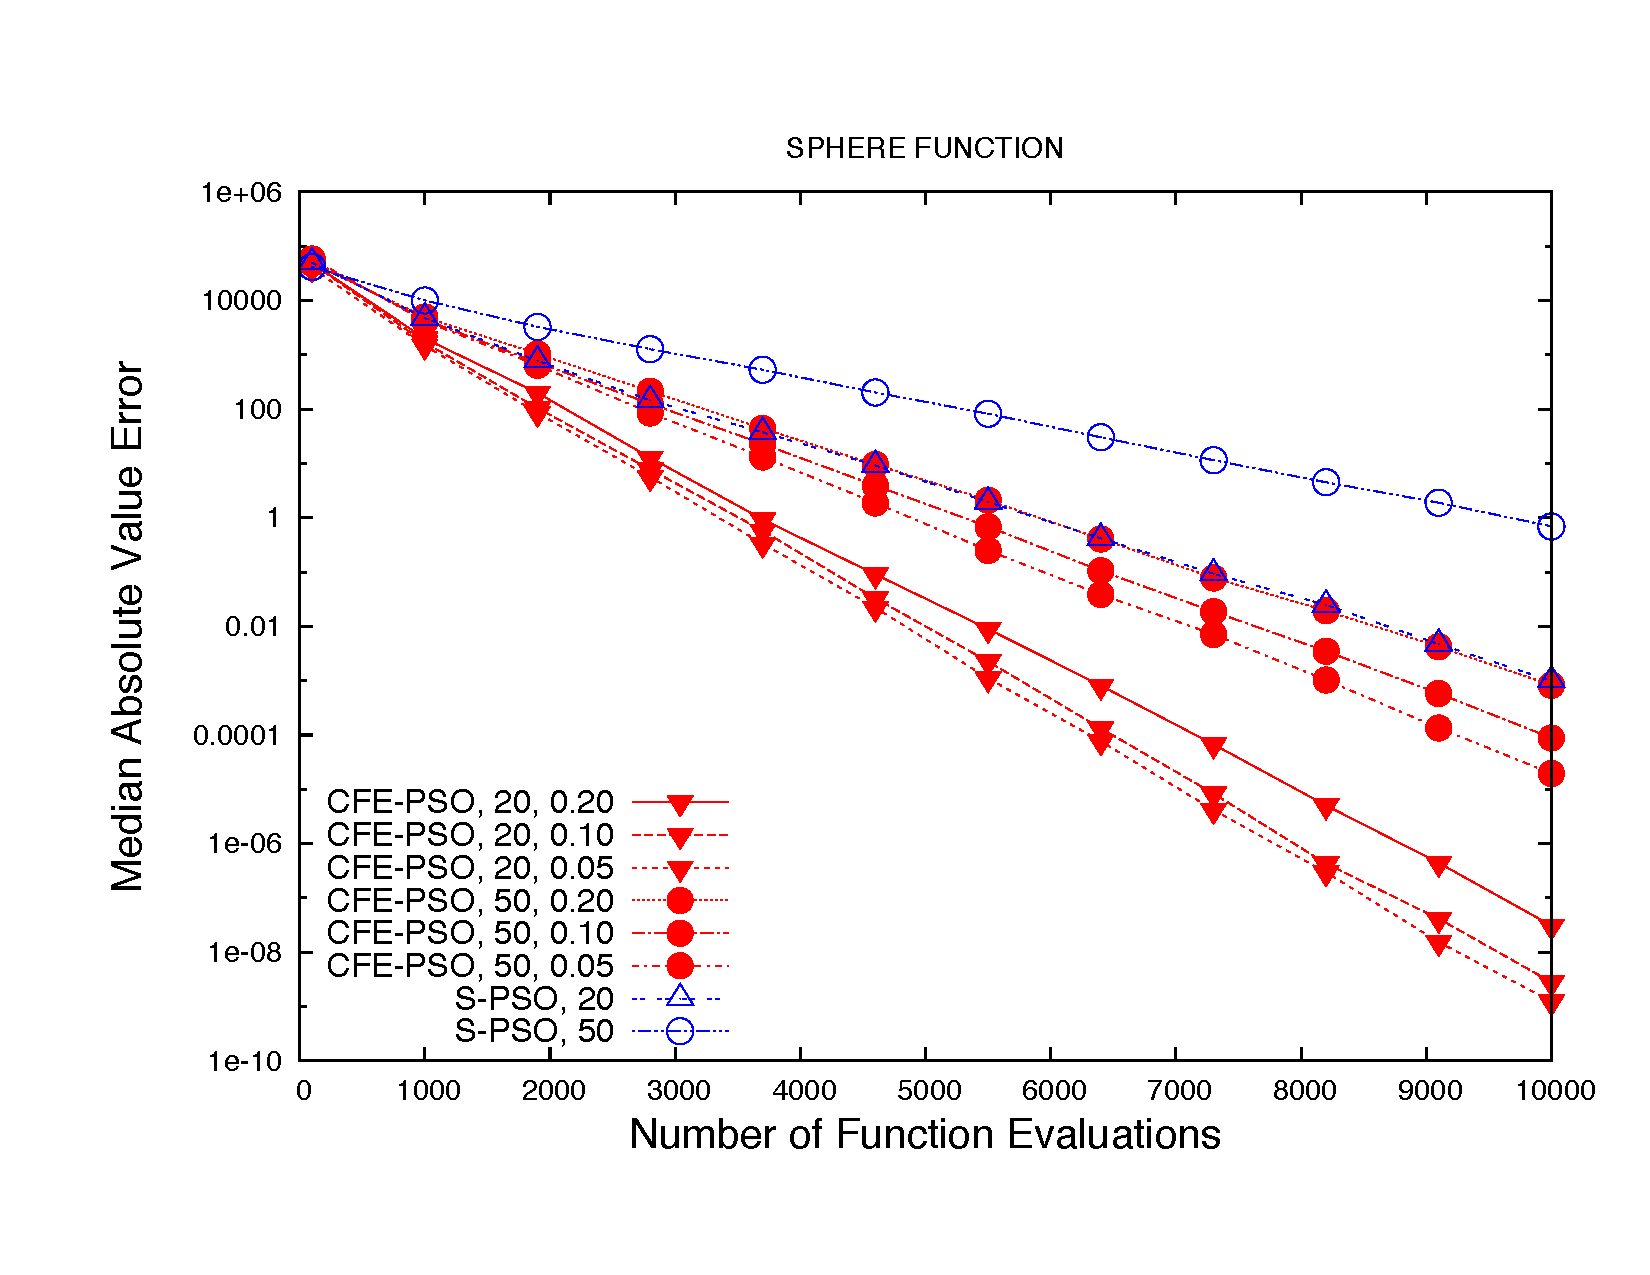
\includegraphics[trim=0.70in 0.8in -0.6in 0in, clip=true, width=3.0in, angle=0]{graphs/sphere-gbest-20-and-50-parts-3-probFEs.pdf}
}
\subfigure[Rosenbrock Function]{
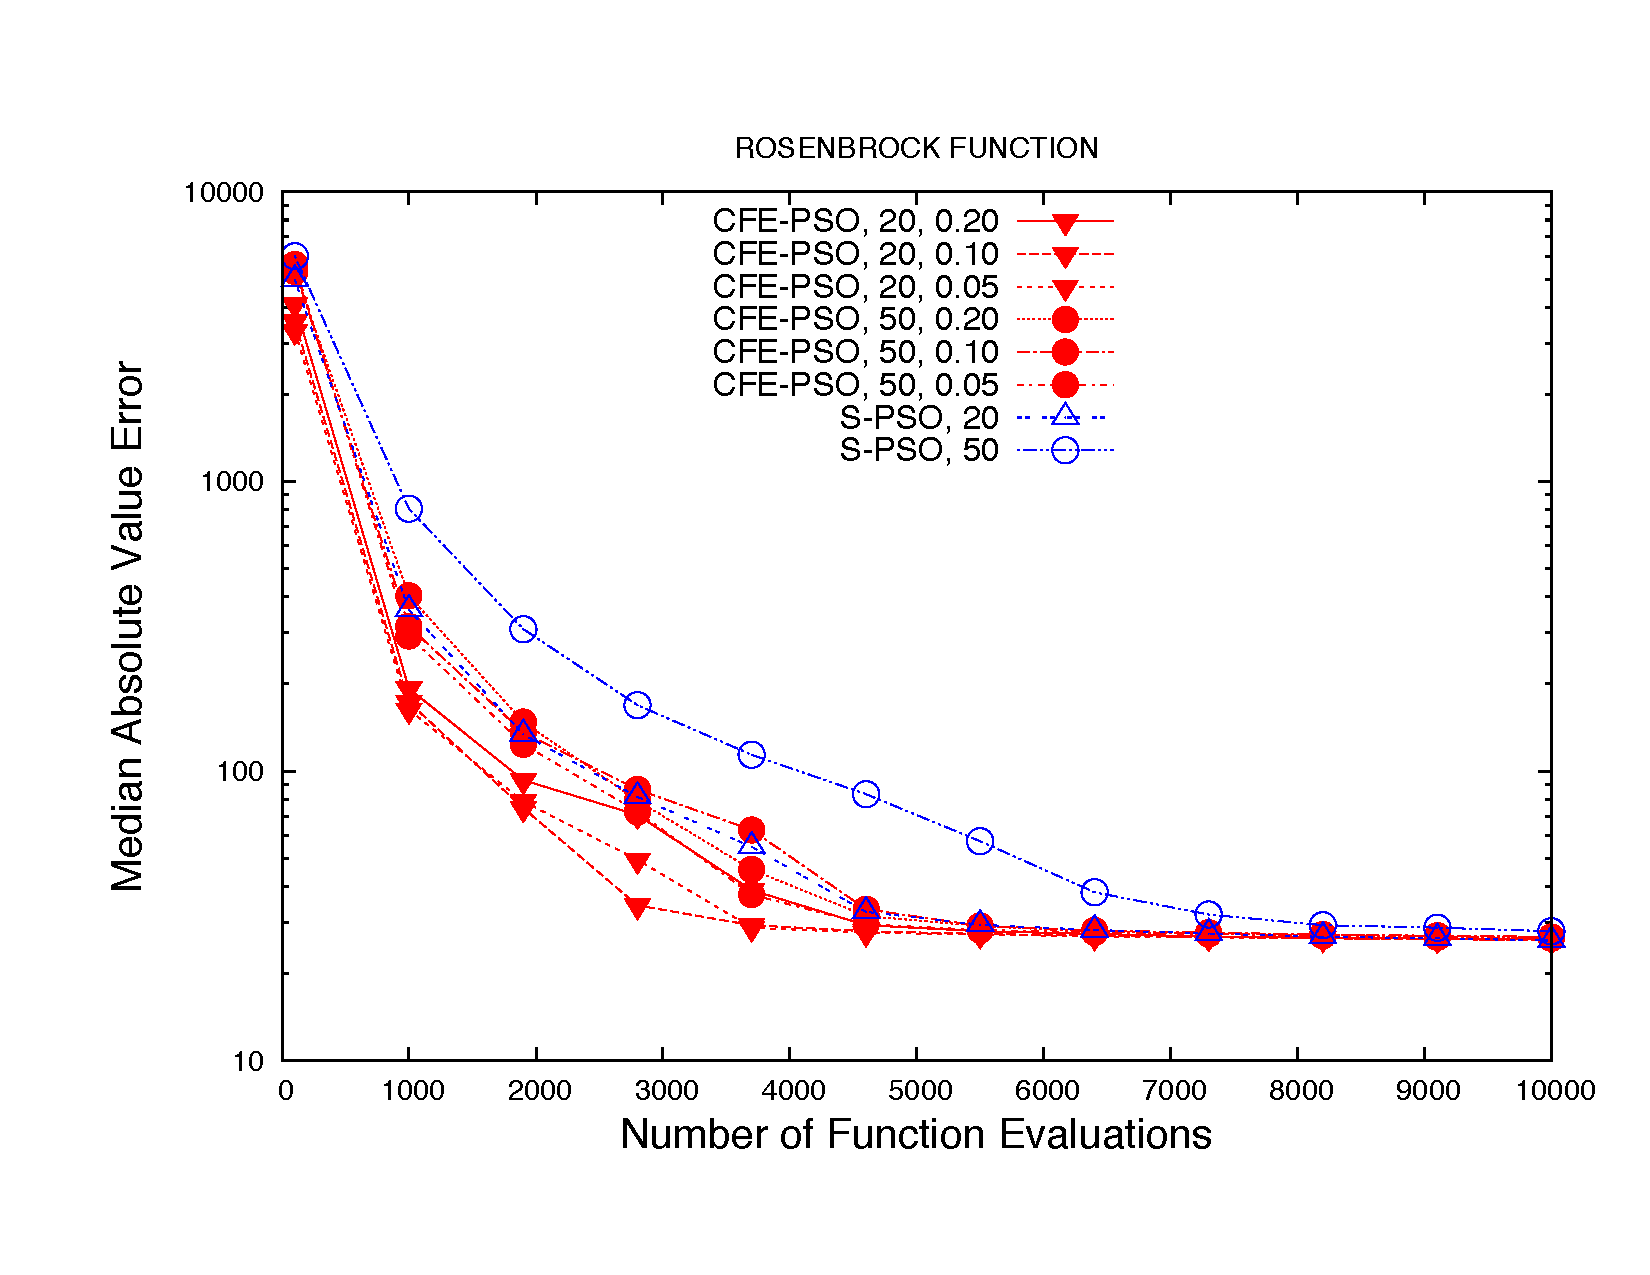
\includegraphics[trim=0.70in 0.8in -0.6in 0in, clip=true, width=3.0in, angle=0]{graphs/rosenbrock-gbest-20-and-50-parts-3-probFEs.pdf}
}
\subfigure[Ackley Function]{
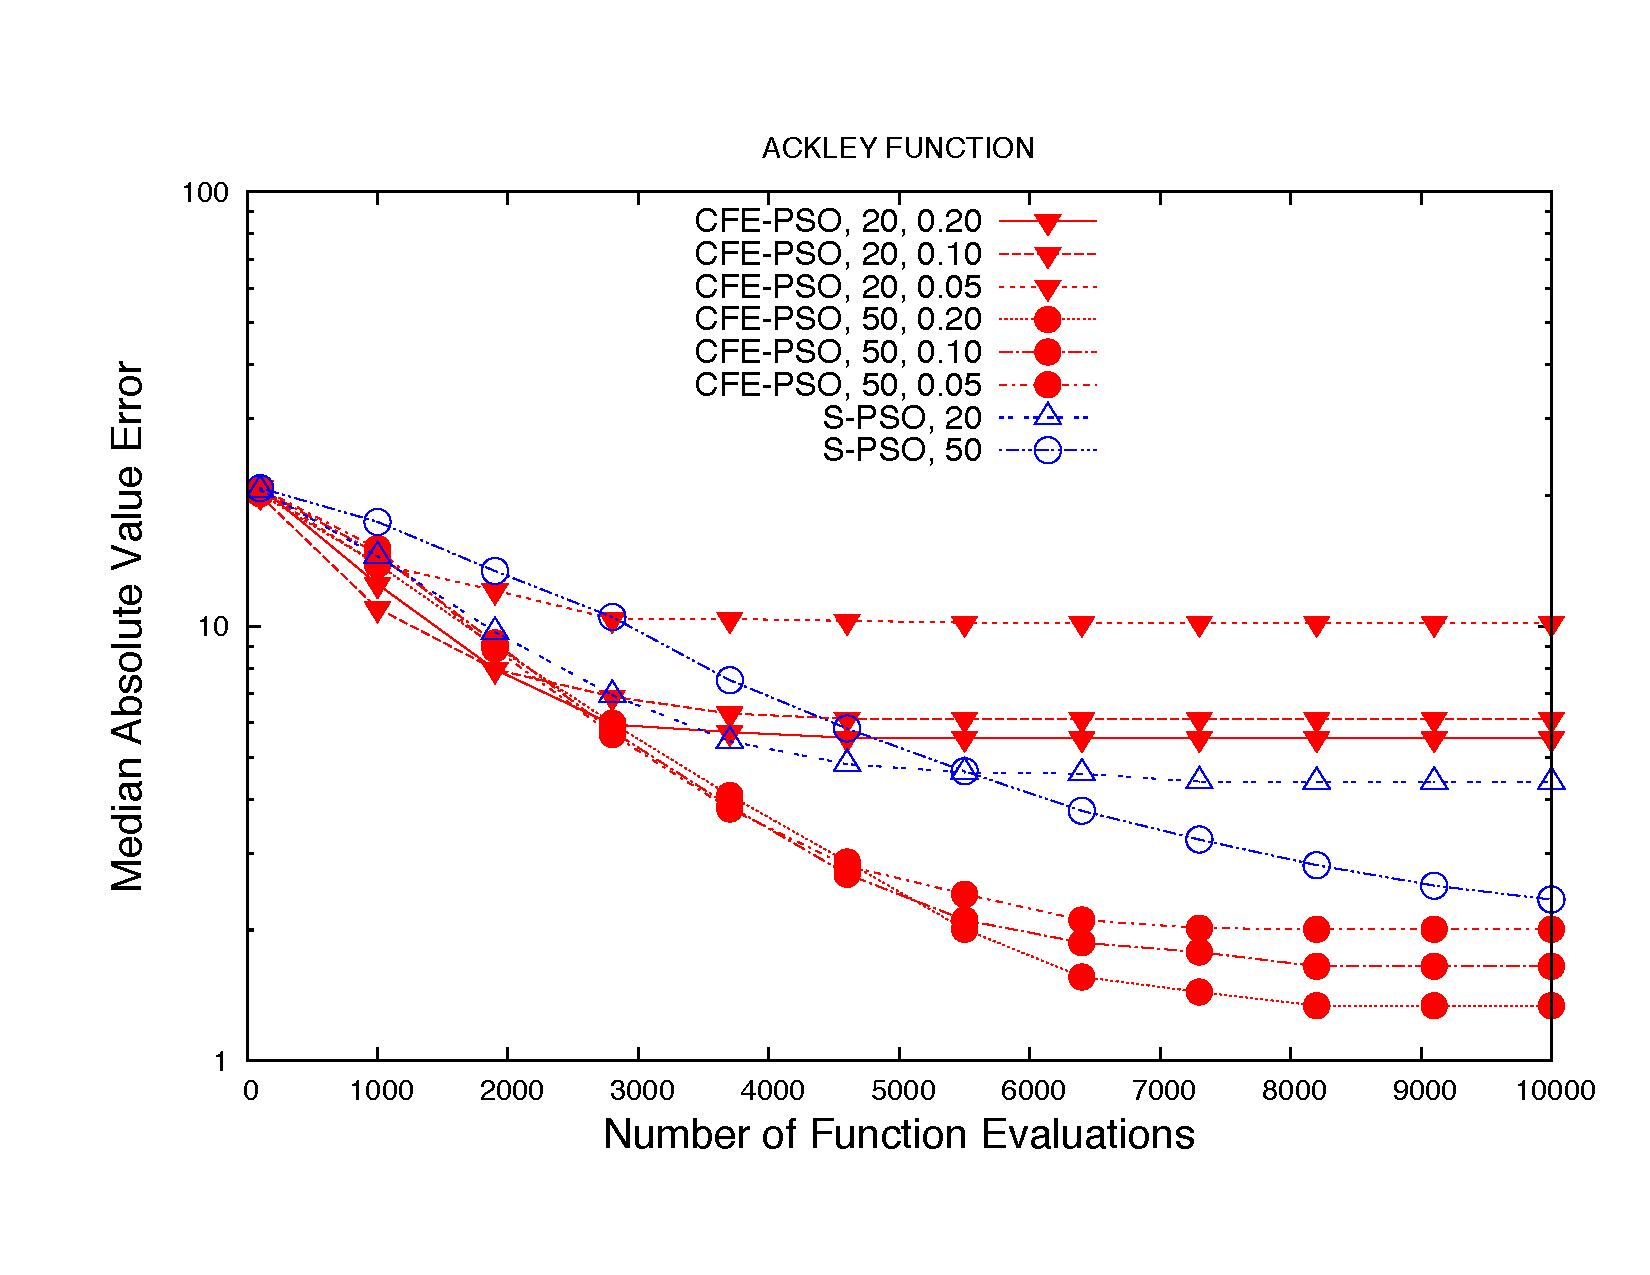
\includegraphics[trim=0.70in 0.8in -0.6in 0in, clip=true, width=3.0in, angle=0]{graphs/ackley-gbest-20-and-50-parts-3-probFEs.pdf}
}
\subfigure[Griewank Function]{
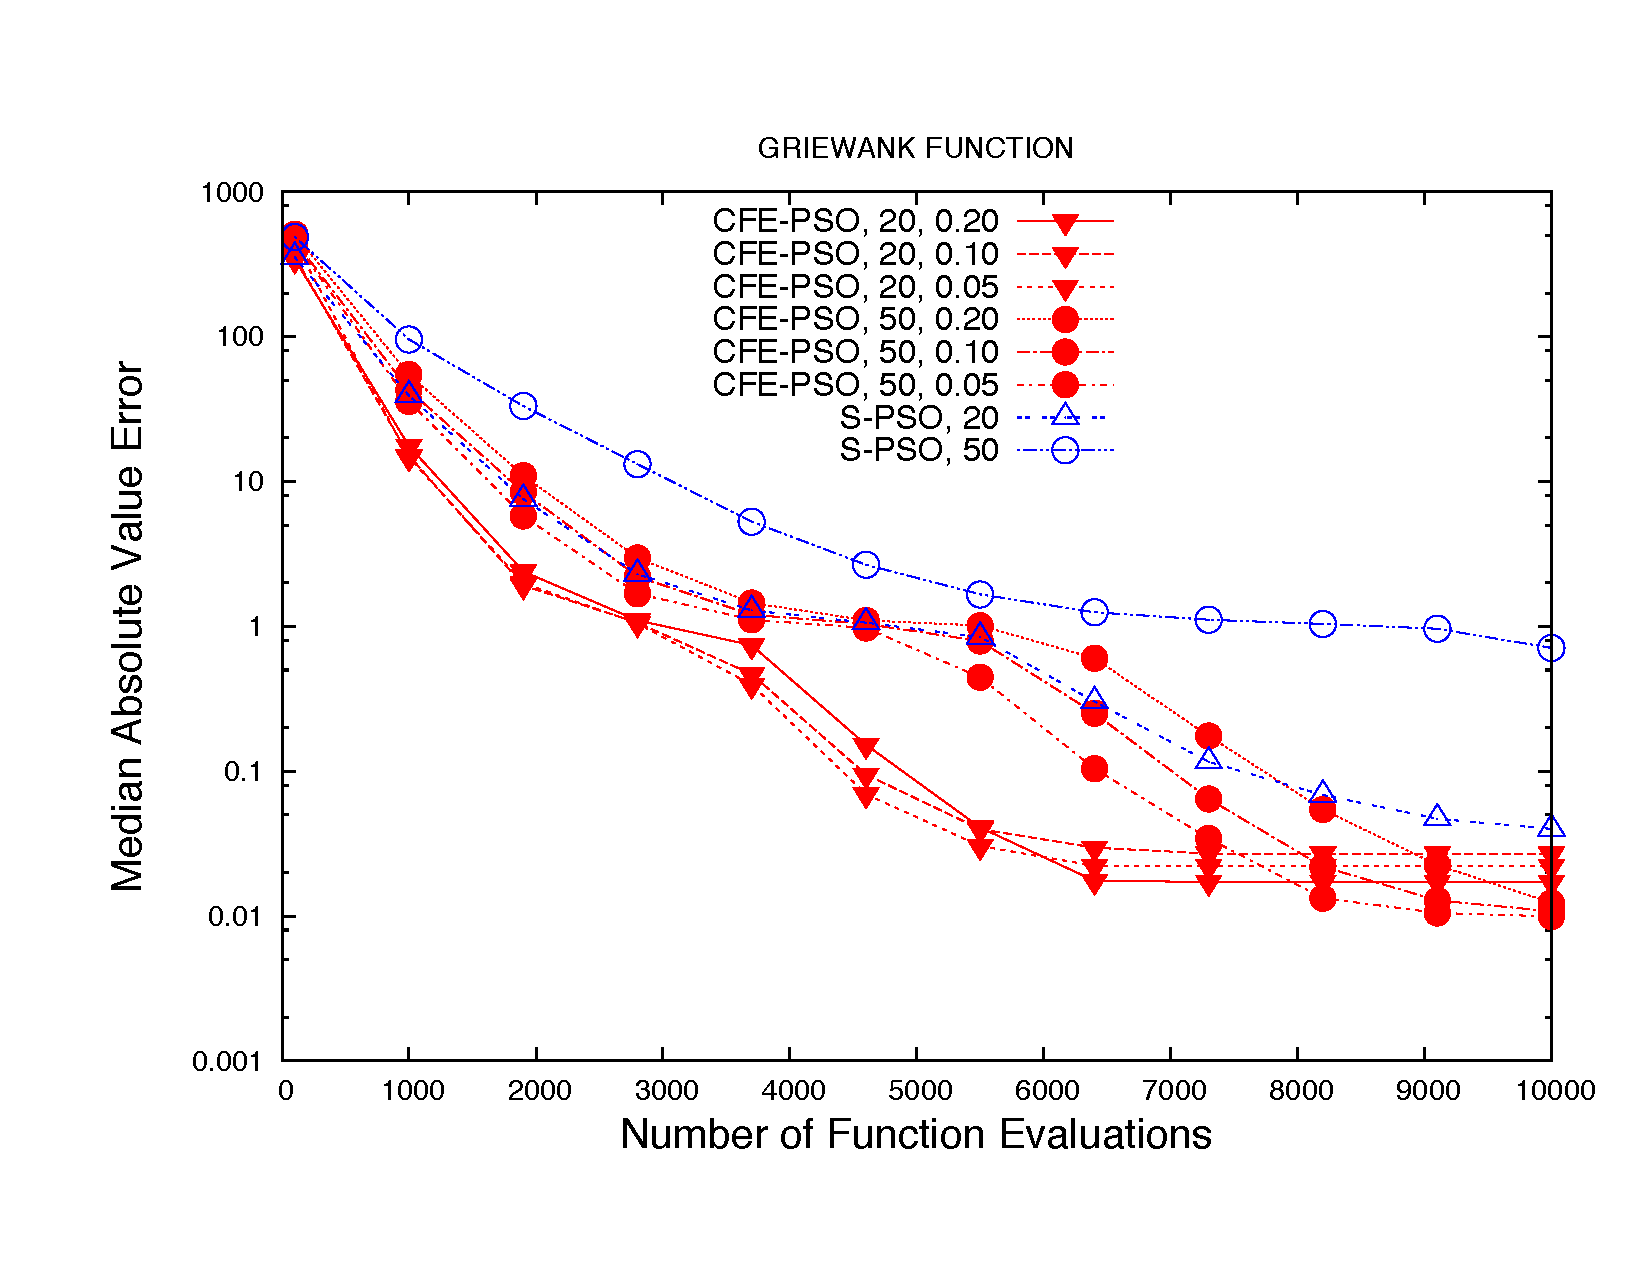
\includegraphics[trim=0.70in 0.8in -0.6in 0in, clip=true, width=3.0in, angle=0]{graphs/griewank-gbest-20-and-50-parts-3-probFEs.pdf}
}
\subfigure[Rastrigin Function]{
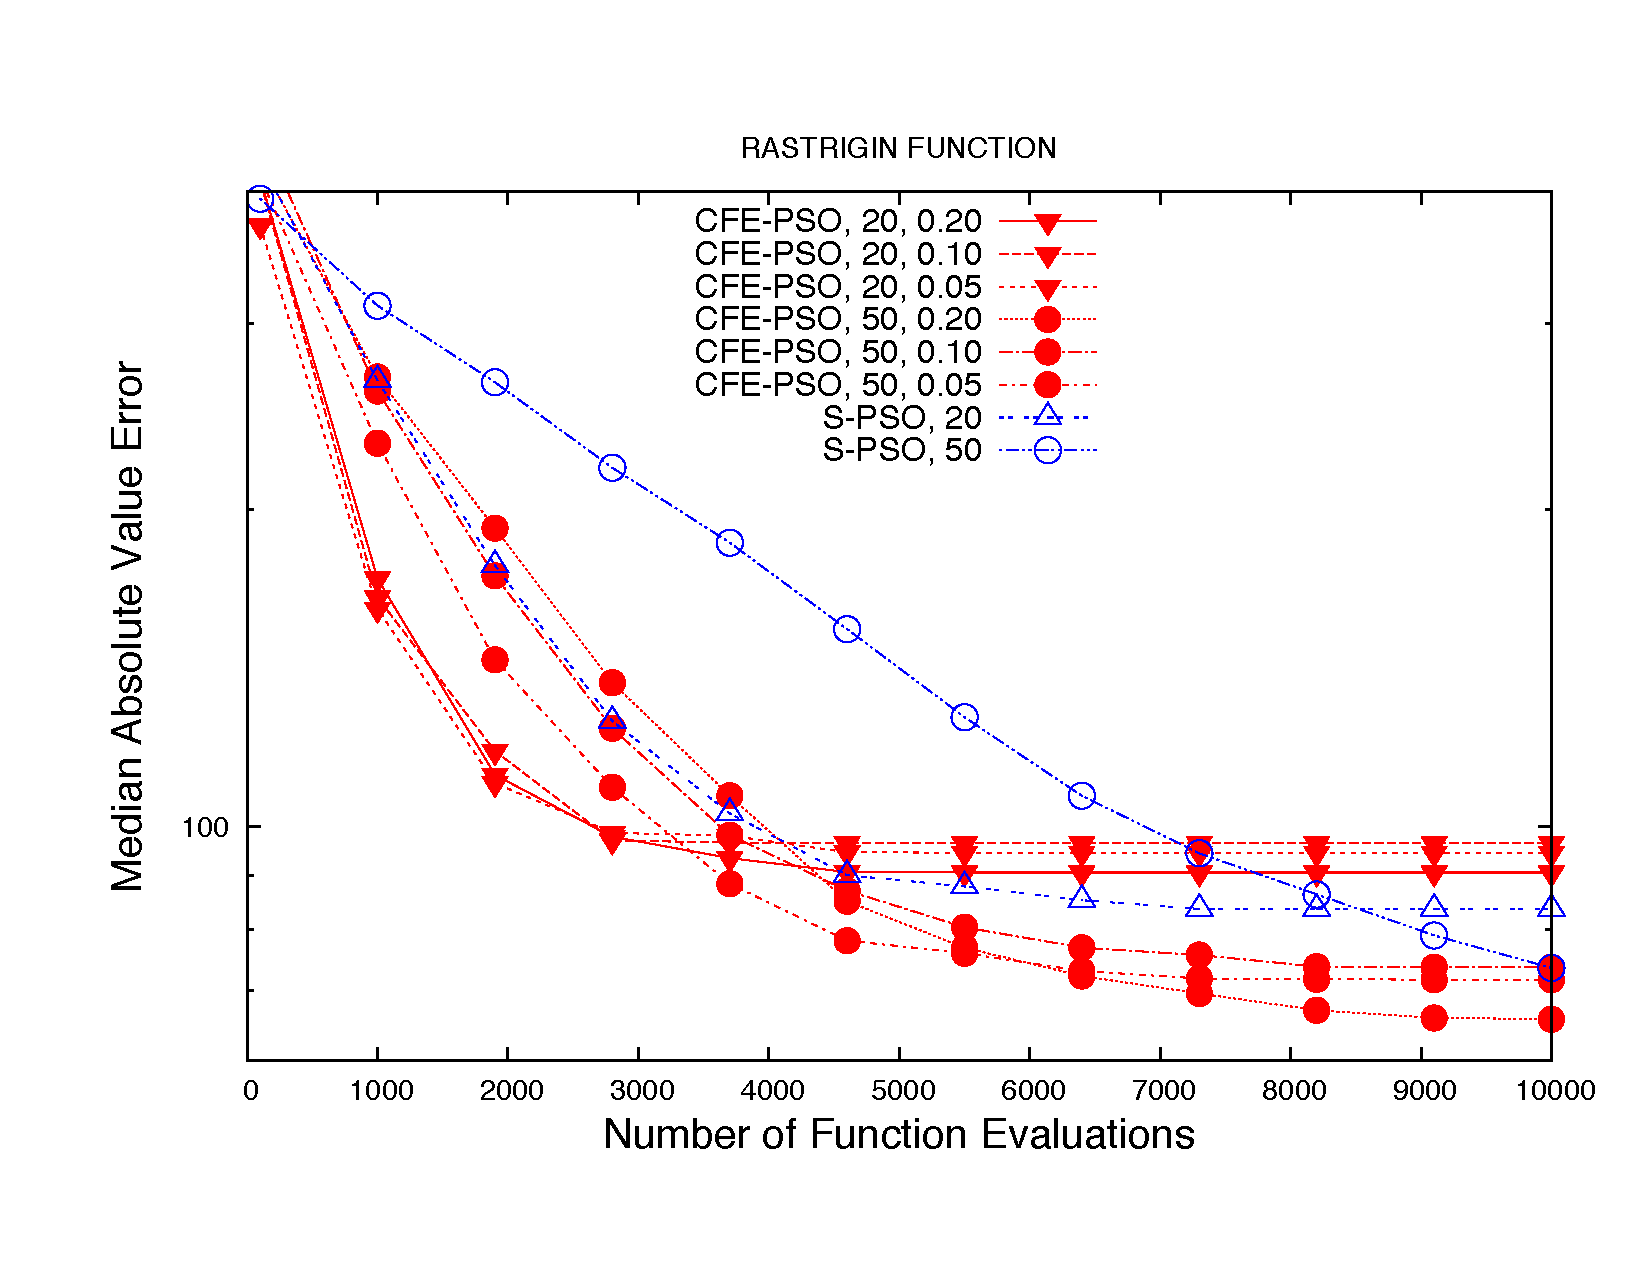
\includegraphics[trim=0.70in 0.8in -0.6in 0in, clip=true, width=3.0in, angle=0]{graphs/rastrigin-gbest-20-and-50-parts-3-probFEs.pdf}
}
\subfigure[Penalized Function P16]{
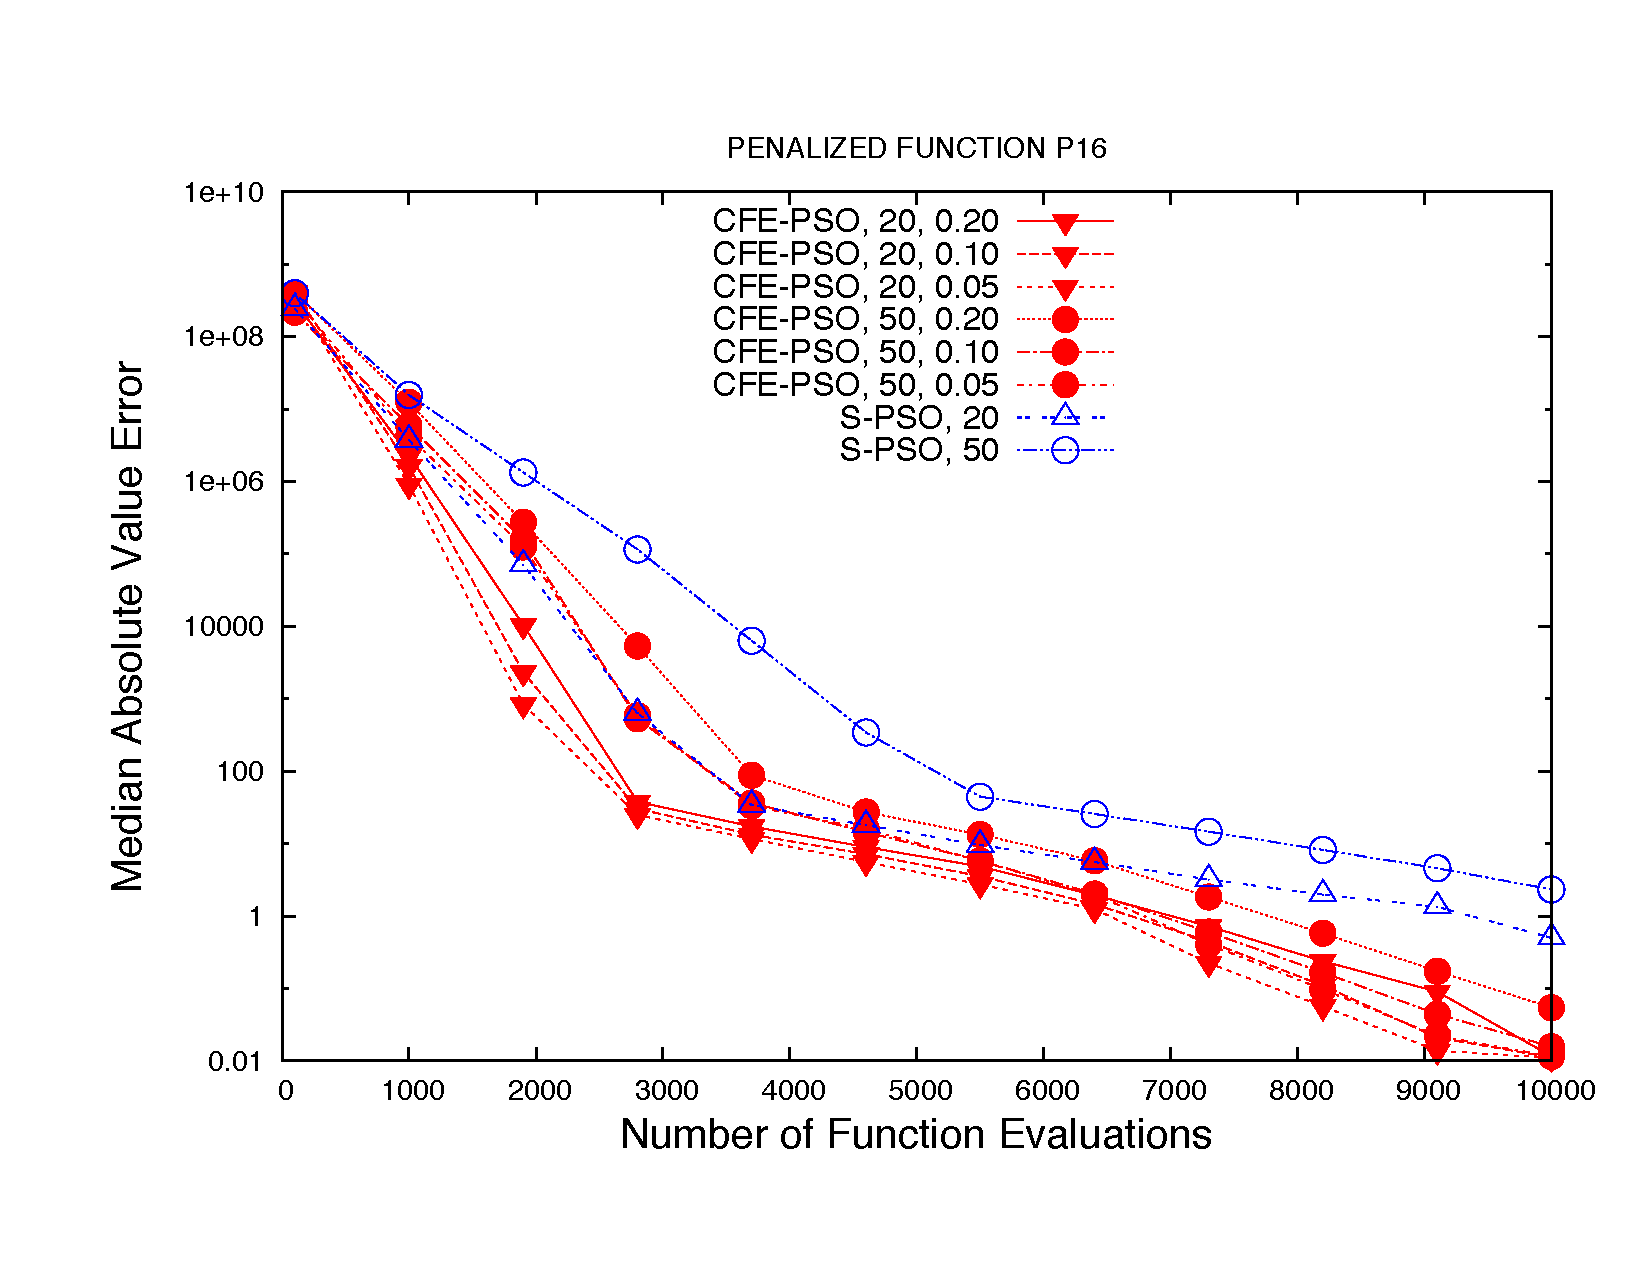
\includegraphics[trim=0.70in 0.8in -0.6in 0in, clip=true, width=3.0in, angle=0]{graphs/penal-p16-gbest-20-and-50-parts-3-probFEs.pdf}
}
\caption{Comparison of \cfe\ and \spso: median absolute value error (log scale) as a function of number of \fes}
\label{f:gbest-graphs}
\end{figure*}


Given a swarm with 20 or 50 particles, the improvement in performance was most pronounced at or below a \pfe\ of 0.5.  The performance showed a tendency to improve as \pfe\ decreased, so we tested  two values below 0.1, i.e.\ 0.05 and 0.01.  While a \pfe\ of 0.05 often produced results that were better than those with a \pfe\ of 0.1, a \pfe\ of 0.01 was almost never better than a \pfe\ of 0.05.  In addition, since \cfe\ reduces the number of \fes\ on each iteration by a factor of \pfe, the run time increases by a factor of 1/\pfe, and the additional run time with a \pfe\ of 0.01 did not justify the occasional improvement in performance.  The best results for 20-particle and 50-particle swarms were obtained with a \pfe\ of 0.2, 0.1, or 0.05. Thus, we show results for these six \cfe\ cases and for \spso\ with 20 particles and 50 particles.

Results for the six versions of \cfe\ and the two versions of \spso\ are presented in Table~\ref{t:gbest-data} and Figure~\ref{f:gbest-graphs}.  For each function, the results from the six \cfe\ \algs\ are followed by those from the two \spso\ \algs. The mean and standard deviation of the lowest function value found are shown in Table~\ref{t:gbest-data}.  To show the reduction in error during the run, we report the median error  at intervals of 2,000 \fes, also in Table~\ref{t:gbest-data}.  For each function, in each column, the best result is in bold-face and is italicized, and the two next best results are in bold-face. 

In all cases, \cfe\ achieves the lowest average function value, and in all but three cases---Rosenbrock ($f_2$), Ackley ($f_3$) and Rastrigin ($f_5$)---the best three results are all achieved by \cfe.  With the exception of Ackley ($f_3$) and Rastrigin ($f_5$), the \algs\ with the best three average function values also have the lowest standard deviations. In three cases---Sphere ($f_1$), Griewank ($f_4$), and Penalized  P16 ($f_6$)---the two \spso\ \algs\ have the worst average function values. 

In the case of Sphere ($f_1$), the average function value of the best \cfe\ \alg\ (20 particles and \pfe\ of 0.1) was five orders of magnitude better than that of the best \spso\ \alg\ (20 particles).  And, in the case of Penalized P16 ($f_6$), the average function value of the best \cfe\ \alg\ (50 particles and \pfe\ of 0.05) was an order of magnitude better than that of the best \spso\ \alg\ (20 particles). In the other four functions, the performance of the best \cfe\ \alg\ and the best \spso\ \alg\ had the same order of magnitude, but we feel that the proper perspective here is not that the difference is small, but that, in spite of not performing \fncevals\ at every opportunity,
even to the point where the expected number of particles doing a \fe\ during an iteration was only one particle (20 particles with a \pfe\ of 0.05), the performance of \cfe\ was no worse than \spso.

Final median error showed similar results, with \cfe\ showing the lowest median error in all cases but  Rosenbrock  ($f_2$).  In all but two cases---Rosenbrock  ($f_2$) and  Rastrigin  ($f_5$)---the \algs\ that achieved the three lowest final median errors were \cfe\ \algs.  And at every \fe\ milestone, the \algs\ with the three lowest median error were all \cfe\ \algs.  More importantly, the best \cfe\ \alg\ reduced the median error more quickly in two cases---Sphere  ($f_1$) and  Grieweank  ($f_4$)---than the best \spso\ \alg\ (Figure\ref{f:gbest-graphs}).  In  Sphere  ($f_1$), this was true throughout the run, and in  Grieweank  ($f_4$), this was true from approximately \fe\ 3000 to \fe\ 5500. (See Figure~\ref{f:gbest-graphs}.)

None of the six \cfe\ \algs\ tested was the best in all cases, but the results indicate that, over the range of values we tested, the number of particles is a more significant factor than the value of \pfe; for all the functions, changing  the value of \pfe\ does not seem to make a significant difference.  With the exception of  Ackley  ($f_3$), the 20-particle \cfe\ has better performance than the 50-particle \cfe, in terms of median error, until at least approximately \fe\ 3,500.  For the Sphere Function ($f_1$), that difference persists throughout the run, and for  Griewank  ($f_4$) and the Penalized Function P8 ($f_6$), that difference persists until approximately \fe\ 7500 and \fe\ 5500, respectively.  Thus, these results suggest that while a minimum number of particles is necessary to explore the solution space (more than 10, given our initial explorations described above), a smaller swarm can explore the space sufficiently, and the increased number of iterations made possible by the smaller swarm, more than compensates for the size of the swarm.

The final errors for the 121 runs for the best \cfe\ \alg\ and the best \spso\ \alg\ for each function were rank ordered and a 2-tailed Mann-Whitney U-test was used to compare the ranks. Since the samples were large enough ($> 20$), the distribution of the U statistic approximates a normal distribution, so we report the Z-score, which is typically used in such cases, as well as the U-score. The results indicate a statistically significant difference in the distributions of the two groups at the 0.01 level---the error of the \cfe\ tests being less than that of the \spso\ tests---for four of the test functions:  Sphere ($f_1$), Ackley ($f_3$), Griewank ($f_4$), and Penal P16 ($f_6$).
The results indicated that there was not a statistically significant difference for two of the functions: Rosenbrock ($f_2$) and Rastrigin ($f_5$).
See Table~\ref{t:mann-whitney-data}.



\begin{table}
\begin{tabular}{|| l | r | r | r | r | r ||}

\hline \hline 

    &   \multicolumn{2}{c|}{Mean Rank}  & &  & \\
                                                                      \cline{2-3}
  Fnc   &     \multicolumn{1}{c|}{\cfe}           & \multicolumn{1}{c|}{\spso}    & \multicolumn{1}{c|}{U}         &   \multicolumn{1}{c|}{Z}     &    \multicolumn{1}{c||}{p}    \\

\hline \hline 

%  SPHERE
$f_1$       &  60.5              &  181.0      &   1    &  -13.44         &  0.0  \\

\hline

% ROSENBROCK       
$f_2$     &  119.6              &  123.5     &   7084     &  -0.43         &  0.67  \\

\hline


%   ACKLEY
$f_3$     &  93.3              &  149.7      &   3913    &  -6.26         &  0.0  \\

\hline

% GRIEWANK
$f_4$     &  90.5              &  152.5      &   3570    &  -6.89         &  0.0  \\

\hline

%   RASTRIGIN
$f_5$     &  115.5              &  127.5     &    6592    &  -1.34         &  0.18  \\

\hline

%   PENAL 2  (P16)           
$f_6$     &  85.6              &  157.4      &   2977    &  -7.98         &  0.0  \\

\hline \hline


\end{tabular}
\caption{Mann-Whitney statistics for final errors }
\label{t:mann-whitney-data}
\end{table}




\cfe\ can be viewed as an extreme form of fitness inheritance, so we also compared \cfe\ to a \pso\ \alg\ that employs this approach. In fitness inheritance techniques, the value of the objective function for a particle's current position is approximated based on the objective function values of some set of particles designated as its ``parents,'' thereby avoiding function evaluations. In \cfe, a particle that does not do a \fe\ is its own parent, inheriting its own \fe\ directly.

Reyes-Sierra and Coello Coello incorporated fitness inheritance into a \pso\ \alg\ (the only work we are aware of that incorporates fitness inheritance into the \psoalg) and tested the effectiveness of twelve fitness inheritance techniques (and four fitness approximation techniques) in a multi-objective \pso\ \alg~\cite{reyes-sierra07}.  {\sc mopso}, the multi-objective \pso\ \alg\ they test these techniques on, is based on Pareto dominance and, at any given point, there is a set of \emph{leaders}, which are the nondominated solutions. The scope from which these leaders are drawn is the entire swarm, so the topology of their algorithm is similar to the global topology of \cfe.

These leaders, along with the standard personal best of a particle and the previous position of a particle, form the set of possible parents when calculating the fitness inherited by that particle.  We compared \cfe\ to the best three techniques (according to their ranking of overall performance). 
To apply these techniques in a single objective setting, we used the global best for any situation in which a particle from the set of leaders was called for. 

The performance of all three of these approaches was never better than the best \cfe\ population-probability combinations, and, for all functions, the majority of \cfe\ population-probability combinations was 
better than all three of these techniques.
 We note that the differences in performance were, in some cases, quite small.  We are not claiming that \cfe\ is significantly better than these three techniques, but that these three techniques do not seem to be better than \cfe.

It is interesting to note, that the probabilities they tested were equivalent to \cfe\ probabilities in the range of $[0.6,0.9]$, much higher than the function evaluation probabilities we found to be best, i.e.\ in the range of $[0.05,0.2]$.  This supports the idea that in a larger neighborhood, such as the \gbn\ topology, it may be better to do without \emph{any} information for longer periods of time than to use the currently available information, even to approximate objective function values.
 



\section{\uppercase{Additional Related Work}}
\label{s:related-work}

As noted in Section~\ref{s:intro}, there are a number of techniques that seek to avoid expensive function evaluations by approximating the value of the objective function.  These techniques are catalogued and described in~\cite{santana-quintero08} for multi-objective evolutionary algorithms.  Since these techniques have been used primarily in evolutionary algorithms and since the \cfe\ approach is much more closely related to the approximation technique of fitness inheritance, we will not discuss them further.  The work of Reyes-Sierra and Coello Coello is the only work we know of that incorporates fitness inheritance into a \pso\ \alg; that work has been discussed in the previous section.

Akat and Gazi describe a decentralized, asynchronous approach that allows the \pso\ \alg\ to be implemented on multiple processors with very weak requirements on communication between those processors~\cite{akat08b}.  Particles reside on different machines.  At each time step, each particle has access only to some subset of those machines/particles;
thus, there may be significant intervals during which a particle $p$ has received no information from particle $p'$; it may even be the case that, on a given iteration, a particle receives no information from any other particles, in which case its position and velocity remain the same.  
They report that the performance of their approach was comparable to standard \pso\ implementations.  

In other work, Akat and Gazi compared three approaches to creating dynamic neighborhoods 
and suggested that all three approaches were viable alternatives to static neighborhoods~\cite{akat08a}.  
More importantly, however, they considered the effect of the \emph{information flow topology} on the performance of the algorithm.  In the general case, the parameter determining neighborhood composition for each approach is different for each particle, resulting in non-reciprocal neighborhoods, which can be represented as directed graphs. If these digraphs are strongly connected \emph{over time}, i.e.\ if there is a fixed interval such that the union of the digraphs over every interval of iterations of that length is strongly connected, then information flow in the swarm will be preserved and every particle eventually has access to the information gathered by every other particle. 

This  work suggests the possibility that  \cfe\ is creating temporary, smaller neighborhoods, the inhabitants of which are constantly changing, but that are connected over time.  Perhaps the probability of doing a function evaluation is regulating the connectedness of these shifting neighborhoods. An investigation into this possibility could shed light on the performance of \cfe\ and the performance of \pso\ algorithms that use dynamic neighborhoods, in general.

Finally, our results suggest an intriguing relationship with work of Garc\'{\i}a-Nieto and Alba. In~\cite{garcia-nieto12}, they tested a variant of the \spso\ \alg\ in which the neighborhood for each particle on each iteration is constructed by choosing $k$ other particles, or ``informants,'' randomly.  They tested the algorithm over a range of values for $k$ and found evidence for a quasi-optimal neighborhood size of approximately 6. In a sense, the expected number of particles doing \fncevals\ in \cfe\ during an iteration can be viewed as the number of informants for every particle in each iteration, since it is these particles that could potentially provide new information.  If we rank the performance of the \cfe\ \algs, and count the number of times each one appeared in the top five best-performing \algs\ for each test function, we find that the best three are 20 particles with \pfe\ of 0.2, 50 particles with \pfe\ of 0.1, and 50 particles with \pfe\ of 0.05, with an expected number of particles doing \fncevals\ on each iteration of 4, 5, and 2.5, respectively.  This suggests that there might be an optimal range for the expected number of particles doing \fncevals\ during an iteration, and that this range may be similar to the optimal range for the number of informants in the work of Garc\'{\i}a-Nieto and Alba.







\section{\uppercase{Conclusions and Further Work}}
\label{s:future-work}

We have presented \cfe, a \psoalg\ that conserves \fncevals\ by probabilistically choosing a subset of particles smaller than the entire swarm on each iteration and allowing only those particles to perform \fncevals.  The \fncevals\ conserved in this fashion are used to increase the number of particles in the swarm and/or the number of iterations. In spite of the potential loss of information resulting from this restriction on the use of \fncevals, \cfe\ performs as well as, or better than, the standard \psoalg\ on a set of standard benchmark functions.


\cfe\ also provides a novel way to control exploration and exploitation. Given a lower probability of doing function evaluations, information about new global and personal bests is delayed and
the balance is tipped away from exploitation toward exploration.  This opens up the possibility of using \pfe\ as a mechanism to dynamically adjust the relative levels of exploration and exploitation in response to the behavior of the swarm.


The conservation technique we tested is very simple; there are many possibilities for more sophisticated conservation mechanisms.  It is possible that adaptive approaches that take into account various factors, such as the recent history of the particle and the status of other particles in the particle's neighborhood, could improve performance.  For example, perhaps a particle should decide whether to skip a \fnceval\ based on the distance it has moved and/or the change in its function value in the last $k$ moves.  
Another possibility that would still conserve function evaluations, but allow particles to possibly recover missed personal bests, would be for each particle to save the $k$ most recent positions for which it did not do a function evaluation, then pick one of those randomly and evaluate it, adopting it as its personal best if it is better than its current personal best.


Perhaps more importantly, however, the idea of conserving \fncevals\ suggests that it would be fruitful to think of \fncevals\ as a scarce resource that needs to be allocated over time.  This opens up the possibility  of incorporating game-theoretic mechanisms for resource allocation into the \pso\ framework.  For example, an auction mechanism could be used to allocate \fncevals\ either to individuals, or to  neighborhoods that would, in turn, allocate them to the individuals in those neighborhoods. The amount of ``money'' that a particle has for bidding purposes could depend on many things:  for example, how good its current solution is, the trend of its personal best values, and the number of new neighborhood bests it has been responsible for over some period of time. A neighborhood could acquire resources for bidding that depend on similar factors, as well as how good its best is compared to the bests of other neighborhoods.  






\bibliographystyle{apalike}
{\small \bibliography{references}}

\end{document}





